%!TEX root = ../main/main.tex

We can observe that the Strahler number is similar to a centrality measure, in a sense which, is a function who takes a node an assigns a score (with certain conditions), that's why the co-relation between Strahler number is visible. We can define the centrality measure using Strahler number in which sense, a higher Strahler number means higher centrality, it's important to remember that a potential function tell us if a centrality measure is able to root trees, in other words, if a centrality measure admits a potential function, it will roots trees if and only if the potential function is simetric (not necessarily works backwards). It is valid to inquire if this centrality roots trees, we can approach this by defining a a potential function, taking the concept of Strahler number we will take a potential function :

    \begin{equation}
        f_{S_{N}} (v,T) = \left\{ \begin{array}{llc}
             1 &   \text{If v is a leaf (does not have childs)}  &\\
             \\ i & \text{if v has one child with  $f_{S_{N}} = i$, and all other children have  $f_{S_{N}} < i$} \\
             \\ i + 1 &  \text{If v has two or more children with $f_{S_{N}} = i$ and no other children with $f_{S_{N}} > i$} \\
             \end{array}
   \right.
    \end{equation}
    
We can see that this potential function makes sense because the potential of a node it depends of their childs (by definition of Strahler number).

We can see now if this function is symmetric knowing that the concept of the Strahler number, is to represent a directed graph and measure the centrality to different contexts. We can make a counter-example for this and observe that if we consider:
\begin{center}
        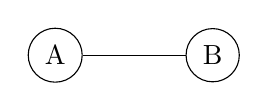
\begin{tikzpicture}
        \node[circle, draw] (A) at (0,0) {A};
        \node[circle, draw] (B) at (2,0) {B};

        \draw (A) -- (B);

    \end{tikzpicture}
\end{center}

In this example we can observe that the centrality goes to the center in the way of A to B and D to C, such that, $f(A,T_{A,B}) =  f(B,T) = 0$ in such way that this is not symmetrical and in this sense does not root trees.

Knowing that this admits a potential function f and f is not symmetrical, by theorem it will not root trees, in other words, we can not find the root of tree in all cases with this centrality. If this centrality does not roots trees we can explore other things like if this potential function in a monoids version, such thing can't because we can observe that, this potencial function implies a monoid that is not associtative (which is not a monoid by definition), such leaf function can be drafted like:
\begin{equation}
    \max\{ x,y \}= \left\{ \begin{array}{lcc}
              \max\{x,y \} &   if  & x \neq y \\
             \\ \max\{ x,y \} + 1 & if  & x = y 
             \end{array}
   \right.
\end{equation}
This function can represent correctly the centrality of a single vertex , but, it can not represent a potential function (recursively) because is not associative (and thus is not a monoid), let an example be
\begin{equation}
    \max\{ 1,\max\{ 1,2 \} \} = 2 \\
    \vspace{0.5cm}
    \max\{ \max\{ 1,1 \},2 \}  = 3 \\
    \vspace{0.5cm}
    \rightarrow 2 \neq 3
\end{equation}

If this centrality can not root trees this means, we can not find a root for a tree T, which can be a problem in different aplications.


